\documentclass[conference]{IEEEtran}
\usepackage{amsmath,amssymb}
\usepackage{graphicx}
\usepackage{hyperref}
\usepackage{cite}
\usepackage{float}

\title{A Review of Linux Security Architecture}
\author{
    \IEEEauthorblockN{Mohammad Mahdi Ahmadi}
    \IEEEauthorblockA{
        Instructor: Zeinab Aghaei \\
        \textit{Department of Electrical and Computer Engineering} \\
        \textit{Isfahan University of Technology}\\
        mohammadmahdi\_ahmadi@ec.iut.ac.ir
    }
}

\begin{document}

\maketitle

\begin{abstract}
The Linux operating system is globally renowned for its robust security mechanisms, making it a preferred choice for server environments and mission-critical applications. This paper presents a comprehensive review of the Linux security architecture, focusing on key aspects such as user management, file permissions, network security, and kernel security through modules like SELinux. Additionally, we explore encryption mechanisms and firewalls that safeguard data integrity and confidentiality. The analysis aims to provide insights into Linux's layered security model and its effectiveness in mitigating common threats and vulnerabilities, thereby ensuring system resilience and stability.
\end{abstract}

\begin{IEEEkeywords}
Linux Security, User Management, Kernel Security, File Permissions, SELinux, Cryptography.
\end{IEEEkeywords}

\section{Introduction}
Linux is one of the most widely deployed operating systems, particularly in server and enterprise environments, where security and stability are paramount \cite{liquid-web}. Its open-source nature allows developers to continually innovate and strengthen its security posture \cite{linux-training}. As cyber threats evolve, the demand for a secure, resilient system grows, making Linux’s security features essential for modern computing infrastructures.

This paper provides an in-depth examination of the Linux security architecture, highlighting its core components: user management, file security, network security, and kernel-level protection. Linux implements a layered security approach, where each layer offers specialized mechanisms to protect against unauthorized access, data breaches, and system exploitation. The user management system governs permissions and access control, while file security mechanisms ensure the integrity and confidentiality of stored data. Network security configurations, such as firewalls and encryption, prevent external threats from penetrating the system, and kernel security modules like SELinux enforce strict policy controls at the core of the operating system.

This review aims to elucidate how Linux achieves its high level of security by analyzing each component's role in building a robust defense-in-depth strategy.


\section{User Management System}

Linux offers three primary types of user accounts:

\begin{enumerate}
    \item \textbf{Regular User Account}: A general account with limited access.
    \item \textbf{System Account}: Used by software, such as MySQL, mail services, etc.
    \item \textbf{Root Account}: The system administrator account with unlimited access.
\end{enumerate}

This section introduces six essential Linux commands to manage users:

\begin{enumerate}
    \item \textbf{Create User}
    \item \textbf{Delete User}
    \item \textbf{User Information}
    \item \textbf{List All Users}
    \item \textbf{Switch Accounts}
    \item \textbf{Modify User Information}
\end{enumerate}

\subsection{User Management Commands}

\begin{enumerate}
    \item \textbf{Create User}: The \texttt{useradd} command is used to add a new user to the system.
    \item \textbf{Delete User}: The \texttt{userdel} command is used to remove a user from the system.
    \item \textbf{User Information}: The \texttt{id} command displays detailed information about a specific user, such as UID, GID, and associated groups.
\end{enumerate}

\subsubsection{Additional Commands}

\begin{enumerate}
    \item \textbf{List All Users}: You can list all system users by examining the \texttt{/etc/passwd} file or by using the \texttt{cut} command.
    \item \textbf{Switch Between Accounts}: The \texttt{su} (switch user) command allows a user to switch between different user accounts.
    \item \textbf{Modify User Information}: The \texttt{usermod} command enables modification of existing user account settings.
\end{enumerate}

\subsection{Password Management}

If you are looking for the file where user information is stored, head directly to \texttt{/etc/passwd}. This file contains details such as usernames, passwords (in encrypted form), home directories, UIDs, and the default shell for each user. However, since this file is readable by all users, it poses a potential security risk in the form of password cracking and dictionary attacks.

To mitigate this risk, Linux employs the shadow password mechanism. When shadow passwords are enabled, the password field in \texttt{/etc/passwd} is replaced with an \texttt{x}, and the actual password hash is stored in the \texttt{/etc/shadow} file. The advantage of this system is that unlike the \texttt{/etc/passwd} file, \texttt{/etc/shadow} can only be accessed by the root user, thus protecting sensitive data from unauthorized access \cite{tldp-authentication}. Furthermore, passwords are stored as cryptographic hashes (not plaintext), typically using the MD5 algorithm.

More details about other cryptographic algorithms in Linux will be discussed in the Cryptography section.

\subsection{Authentication}

So far, we have discussed user management and password storage. But how does the system manage authentication? Where is it determined whether to use encryption or the shadow password method? The answer lies in Pluggable Authentication Modules (PAM).

PAM is the core component of user authentication in all modern Linux distributions. It allows programs like \texttt{su}, \texttt{login}, \texttt{passwd}, and \texttt{xlock} to authenticate users efficiently \cite{tldp-authentication}. The modular structure of PAM ensures transparency and ease in handling different authentication methods without depending on how passwords are stored.

If you need to customize authentication settings, you can edit the configuration files found in the \texttt{/etc/pam.d/} directory. For a deeper understanding of the login process, the article \href{https://www.computerhope.com/unix/ulogin.htm}{Login in Unix} offers further insights. Additionally, login configurations can be found in the \texttt{/etc/login.defs} file.


\section{File Security}

This section covers the fundamentals of file security, including file permissions. To view file information, the command \texttt{ls -l} is used. This command provides details about a file, including its type, permissions for three categories of users (the current user, the group, and others), the owner's name, the file name, the creation date, and more. Additionally, the command \texttt{chown} can be used to change the ownership of a file.

\subsection{Permissions}

The notation \texttt{rwxr-xr-x} or similar strings represent file permissions. When discussing file permissions, this is exactly what is meant. These characters are divided into three groups of three letters, \texttt{r}, \texttt{w}, and \texttt{x}, where each has its own meaning as outlined below \cite{geeksforgeeks-acl}:

\begin{itemize}
    \item \texttt{r} (read): Grants read permission, allowing the file to be read or the directory's contents to be listed.
    \item \texttt{w} (write): Grants write permission, allowing changes to the file or the directory's contents.
    \item \texttt{x} (execute): Grants execute permission, allowing the file to be executed (if it is a program) or access to the directory.
\end{itemize}

These nine characters are divided into three subsets:
\begin{enumerate}
    \item The first three characters represent the permissions for the file owner.
    \item The next three characters represent the permissions for the members of the file's group.
    \item The last three characters represent the permissions for all other users.
\end{enumerate}

To modify a file's permissions, the \texttt{chmod} command can be used. For example, the command \texttt{chmod 777 filename} grants all permissions (read, write, and execute) to the file for all three user categories. Each digit corresponds to a permission set, where the values are determined by summing the permissions: \texttt{r} = 4, \texttt{w} = 2, \texttt{x} = 1. Thus, \texttt{777} means that each group has full permissions.

As illustrated in Figure 1, the numerical representation of the permissions is visualized for better understanding.

\begin{figure}[H]
    \centering
    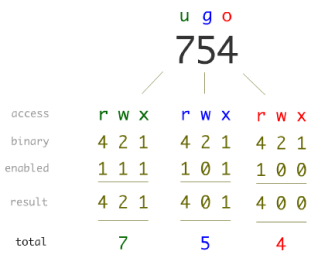
\includegraphics[width=0.4\textwidth]{fig1.jpg}
    \caption{Numerical representation of the permissions \cite{cloudxlab-permissions}.}
    \label{fig:filetypes}
\end{figure}

\subsection{Access Control Lists (ACLs)}

Access Control Lists (ACLs) in Linux provide a more flexible permission management mechanism alongside traditional file permissions. Imagine a scenario where a user is not part of a group but you still want to grant them read or write access to a file without adding them to the group. This is where ACLs come into play.

ACLs allow for more granular control over permissions. According to the Linux manual, ACLs are used to define fine-grained discretionary access rights for files and directories.

For more information on using ACLs in Linux, you can refer to this resource: 
\url{www.geeksforgeeks.org/access-control-listsacl-linux/}.

\section{Network Security}

As the world becomes increasingly connected, network security in Linux gains more importance. Compromising network security is often simpler and more common than compromising physical or local security. Operating systems play a critical role in managing network communications, controlling access, and authenticating users. To counter potential cyber threats, strong security measures such as firewalls, encryption, and intrusion detection systems are implemented. Regular updates and patches are also essential to address vulnerabilities. By employing advanced network security protocols, operating systems can safeguard sensitive data and provide a secure and reliable environment for users.

This section discusses what network security entails and how Linux approaches it.

\subsection{Firewall}

A firewall is a security mechanism—either software or hardware—that prevents unauthorized access to computers by controlling the traffic exchanged over a network. It serves as a filter that data must pass through, ensuring secure communication. The primary goal of a firewall is to separate secure data from untrusted zones and manage interactions between them. While firewalls can perform various tasks, their primary function is to control incoming and outgoing communications between a device and the network.

Software firewalls, often referred to as personal firewalls, are designed for installation on individual computers. They are typically used in homes or small offices that maintain prolonged connections to the internet. These firewalls prevent unauthorized access by detecting and blocking communications over high-risk ports. A firewall acts much like a door in a house: anyone entering or exiting must pass through this point of control. The firewall sits at the gateway of a computer, regulating all network traffic.

\subsection{IPTables}

As is well-known, internet traffic is composed of packets. In a network, data is transmitted in small, fragmented parts called packets. The destination computer reassembles these packets to form the complete data. \textit{iptables} is responsible for identifying these packets and performing specific actions on them based on user-defined rules.

Packet filtering through \textit{iptables} is based on four key concepts \cite{roxo}:

\begin{itemize}
    \item \textbf{Tables:} A table is a collection of chains, where each chain holds a set of rules for managing packets.
    \item \textbf{Chains:} A chain is a sequence of rules, and when the system receives a packet, \textit{iptables} identifies the relevant table and processes the packet through these rules until it finds the appropriate one.
    \item \textbf{Rules:} A rule dictates how the system should handle a specific packet. For example, a rule might instruct the system to block a particular type of packet or allow it to pass.
    \item \textbf{Target:} The target refers to the action that will be taken on a packet, such as accepting, dropping, or rejecting it.
\end{itemize}

Accepting a packet means allowing it to pass through the firewall, dropping a packet means blocking it without notifying the sender, and rejecting a packet sends an error back to the sender, indicating the packet was denied. In the case of dropped packets, no error is returned to the sender. Additionally, returning a packet halts its progression through the current chain and sends it back to a previous chain.

For example, if your server detects multiple attacks from the IP address \texttt{192.168.1.3}, you might want to block all incoming packets from this address. This task is handled by the INPUT chain within the Filter table:

\begin{verbatim}
iptables -A INPUT -s 192.168.1.3 -j DROP
\end{verbatim}

This command will block all incoming packets from the specified IP address.

Additionally, web traffic protocols such as HTTP operate on port 80, HTTPS on port 443, and SSH on port 22. If you wish to allow connections on one of these ports, you would first specify the connection protocol (e.g., TCP) and then define the desired port. For example, enabling traffic on TCP port 22 for SSH:

\begin{verbatim}
iptables -A INPUT -p tcp --dport 22 -j ACCEPT
\end{verbatim}

As shown above, the protocol used is TCP, and \texttt{dport} specifies the target port within the TCP connection.

\section{Kernel Security}

The term \textit{Linux Security Modules} (LSM) refers to a framework that allows the Linux kernel to support various operating system security models without bias. Since Linux kernel version 2.6, LSM has become a standard component of the Linux kernel. Some of the officially accepted security modules within the kernel include AppArmor, SELinux, Smack, and TOMOYO Linux \cite{linux-training}.

In the following section, we will explore the SELinux module in greater detail.

\subsection{SELinux}

\textit{Security-Enhanced Linux} (SELinux) is a security architecture for Linux systems that allows system administrators to exercise more granular control over who can access the system. SELinux was originally developed by the United States National Security Agency (NSA) as a series of patches for the Linux kernel using the LSM framework \cite{geeksforgeeks-acl}. The SELinux module was released to the open-source community in 2000 and integrated into the Linux kernel in 2003.

SELinux defines access controls for applications, processes, and files within a system. It employs security policies, which are a set of rules that determine what can and cannot be accessed by SELinux. When an application or process, known as a \textit{subject}, requests access to an \textit{object}, such as a file, SELinux checks the request against its Access Vector Cache (AVC). The AVC is where the permissions for subjects and objects are stored.

If access is denied, an \texttt{avc: denied} message will be logged in \texttt{/var/log/messages}.

\section{Cryptography in Linux}
The Linux kernel provides a cryptographic API for use by kernel subsystems \cite{sandilands}. This API supports a wide range of cryptographic algorithms, including common symmetric ciphers, hashing functions, and asymmetric cryptography. Both synchronous and asynchronous methods are available, with the latter being particularly useful for hardware-based cryptography, which offloads processing from the CPU.

Cryptography in Linux covers various use cases, such as file encryption with well-known algorithms like the Advanced Encryption Standard (AES), generation and distribution of public and private keys (e.g., Rivest Shamir Adleman, RSA), digital signing of messages, password hashing and storage, among others.

The following sections outline various Linux subsystems and tools that utilize cryptography:

\subsection{Secure Communication Protocols}
Linux supports secure communication protocols such as TLS/SSL (Transport Layer Security/Secure Sockets Layer) to secure data transmission over networks. For example, web servers employ TLS/SSL to encrypt communications over HTTPS.

\subsection{SSH (Secure Shell)}
Linux uses SSH for secure remote access and file transfer between servers. SSH leverages public key cryptography for authentication and symmetric key encryption for secure data exchange.

\subsection{Disk Encryption}
Linux provides disk encryption tools like LUKS and dm-crypt to safeguard data stored on drives \cite{liquid-web}. These tools can encrypt entire drives or specific partitions, ensuring that data remains secure even if physical access to the drive is compromised.

\subsection{GPG (GNU Privacy Guard)}
GPG, which implements the OpenPGP standard, allows users to encrypt and sign files and emails in Linux. This ensures that the principles of confidentiality and data integrity are maintained.

\subsection{File and Folder Encryption}
Linux offers tools such as eCryptfs and EncFS that allow users to encrypt specific files or folders within the filesystem.

\subsection{SSL/TLS Certificates}
Linux stores SSL/TLS certificates used for HTTPS and other secure communications. Certificate Authorities (CAs) issue these certificates to verify the identity of websites and services.

\subsection{Random Number Generation}
Random number generators, such as \texttt{/dev/random} and \texttt{/dev/urandom}, are essential for security-related operations in Linux, including key generation and salting.

\subsection{Hash Functions}
Linux utilizes cryptographic hash functions like SHA-256 for secure password storage and data integrity verification (e.g., Message Authentication Codes, MACs).

\subsection{Package Verification}
Linux package managers, such as APT (Debian/Ubuntu) and RPM (Red Hat/CentOS), use cryptographic signatures to verify the authenticity and integrity of software packages during installation and updates, often through GPG signatures.

\subsection{VPN Support}
Linux supports various VPN protocols, including IPsec and OpenVPN, which utilize cryptography to establish secure tunnels for data transmission.

\subsection{Secure Erasure}
Linux includes tools like \texttt{shred}, which ensures the secure erasure of data by repeatedly overwriting files, making data recovery difficult.

\section{Malware in Linux}
Although Linux is often regarded as more secure than other operating systems, such as Windows, it is not immune to malware \cite{mend}. However, due to its design and robust security measures, malware infections on Linux systems are relatively rare. Despite this, various types of malware can still affect Linux environments. Some common types of malware in Linux include:

\subsection{Trojans}
Linux trojans are malicious software that disguise themselves as legitimate programs. They can be distributed through compromised repositories, infected emails, or incorrect downloads.

\subsection{Rootkits}
Rootkits are malware designed to hide the presence of an intruder on a system. While granting unauthorized access to attackers, they also conceal the attacker’s activities from system administrators and security tools.

\subsection{Backdoors}
Backdoors are programs or code that provide unauthorized access to a system, allowing attackers to bypass normal authentication mechanisms and gain illicit entry into the operating system.

\subsection{Botnets}
Linux systems can become infected and form part of a botnet. Botnets are networks of compromised computers controlled by a hacker for malicious purposes.

\subsection{Ransomware}
Although rare in Linux, ransomware can target vulnerable systems, encrypting important files and demanding ransom for their decryption.

\subsection{Keyloggers}
Keyloggers intercept and record keystrokes, leading to the theft of sensitive information, such as passwords.

\subsection{Spyware}
Spyware is designed to gather information about a user's activities without their knowledge, posing a significant privacy threat.

\subsection{DDoS (Distributed Denial of Service) Attack Tools}
Linux systems can be infected with malware that turns them into botnet zombies, which are then used in distributed DDoS attacks against target websites or networks.

\subsection{Worms}
Linux worms are self-replicating malware that can spread across networks without user intervention, exploiting vulnerabilities to infect other systems.

\subsection{Cryptojacking}
This type of malware utilizes the system’s computing resources to mine cryptocurrency without the owner's consent.

\subsection{Phishing Attacks}
Although not a type of malware, Linux users can fall victim to phishing attacks, where attackers attempt to trick them into revealing sensitive information, such as login credentials.

Users must remain vigilant and practice good security habits, such as keeping systems updated, using strong passwords, and avoiding suspicious downloads or websites. Additionally, utilizing security software and adhering to best practices can further reduce the risk of malware infections in Linux systems.

\section{Digital Forensics}

Digital Forensics involves the process of storing, analyzing, retrieving, and preserving electronic data that may be useful in investigations. This includes information such as precise login and logout histories, commands executed by users, file modifications, and more.

The operating system’s primary responsibility in the initial stage is to log system events \cite{tldp-security}. Important log files in Linux are detailed below:

\begin{itemize}
    \item \texttt{/var/log/syslog/}: This is a general system log file that includes a wide range of messages, such as kernel messages, system events, and various other activities.
    \item \texttt{/var/log/auth.log/}: This file logs authentication-related events, including user logins, failed login attempts, and authentication errors.
    \item \texttt{/var/log/messages/}: Similar to \texttt{syslog}, this file records general system messages and events.
    \item \texttt{/var/log/dmesg/}: Contains kernel buffer messages and provides information about hardware detection and initialization during system boot.
    \item \texttt{/var/log/kern.log/}: Focuses on messages and events related to the kernel.
    \item \texttt{/var/log/lastlog/}: Stores the most recent login information for each user.
    \item \texttt{/var/log/wtmp/}: Logs events related to user logins and logouts.
    \item \texttt{/var/log/btmp/}: Records failed login attempts.
    \item \texttt{/var/log/secure/}: A log file for monitoring security-related events and authentication attempts.
    \item \texttt{/var/log/cron/}: Records information about cron jobs and scheduled tasks.
\end{itemize}

\section{Historical Security Issues in Linux}

This section explores three notable vulnerabilities in Linux throughout its history.

\subsection{CVE-2017-18017}

This vulnerability affects versions prior to 4.11 \cite{mend}. According to the description, the function \texttt{tcpmss\_mangle\_packet} in \texttt{net/netfilter/xt\_TCPMSS.c} can allow attackers to perform a Distributed Denial of Service (DDoS) attack.

\subsection{CVE-2015-8812}

This vulnerability affects versions prior to 4.5 \cite{mend}. There was a serious flaw in \texttt{drivers/infiniband/hw/cxgb3/iwch\_cm.c} of the Linux kernel, which was unable to correctly identify error conditions. This vulnerability allowed remote attackers to execute arbitrary code or cause a DDoS by manipulating crafted packets.

\subsection{CVE-2016-10229}

This vulnerability affects versions prior to 4.5 \cite{mend}. In this case, \texttt{udp.c} allowed attackers to execute arbitrary code through UDP traffic. Specifically, during the execution of a \texttt{recv} system call with the \texttt{MSG\_PEEK} flag, the second variable, checksum, was not securely handled, leading to this vulnerability.

\section{Conclusion}
In conclusion, the Linux security architecture exemplifies a multi-layered approach that safeguards system integrity, confidentiality, and availability. The combination of user management, file permissions, network security, and kernel-level modules like SELinux creates a resilient security posture capable of defending against diverse threats. As cyberattacks continue to evolve, Linux’s adaptability and its growing ecosystem of security tools remain critical in protecting both personal and enterprise-level systems. Future advancements will likely focus on enhancing these existing mechanisms while addressing emerging security challenges. Therefore, continuous research and development are essential for keeping Linux at the forefront of secure operating systems.

\begin{thebibliography}{99}
    \bibitem{antipope}
    \textit{AntiPope}, "Old Linux Shopper: Cryptography," [Online]. Available: \url{http://www.antipope.org/charlie/old/linux/shopper/167.crypto.html}.

    \bibitem{citeseerx}
    \textit{CiteSeerX}, "Document on Linux Security," [Online]. Available: \url{https://citeseerx.ist.psu.edu/document?repid=rep1&type=pdf&doi=77d8eb76ce82e145e211a9ed8c878500d57606f6}.

    \bibitem{cloudxlab-permissions}
    CloudxLab, "Permissions - Numeric," [Online]. Available: \url{https://cloudxlab.com/assessment/displayslide/64/permissions-numeric}. [Accessed: Sept. 8, 2024].
    
    \bibitem{geeksforgeeks-acl}
    \textit{GeeksforGeeks}, "Access Control Lists (ACL) in Linux," [Online]. Available: \url{https://www.geeksforgeeks.org/access-control-listsacl-linux/}.
    
    \bibitem{geeksforgeeks-commands}
    \textit{GeeksforGeeks}, "7 Linux Commands for Managing Users," [Online]. Available: \url{https://www.geeksforgeeks.org/7-linux-commands-for-managing-users/}.
    
    \bibitem{linux-training}
    \textit{Linux Training}, "Linux Security Training," [Online]. Available: \url{https://linux-training.be/linuxsec.pdf}.
    
    \bibitem{liquid-web}
    \textit{Liquid Web}, "Best Operating System for Web Hosting," [Online]. Available: \url{https://www.liquidweb.com/blog/best-operating-system-for-web-hosting/}.
    
    \bibitem{mend}
    \textit{Mend.io}, "Top 10 Linux Kernel Vulnerabilities," [Online]. Available: \url{https://www.mend.io/blog/top-10-linux-kernel-vulnerabilities}.
    
    \bibitem{openai-chat}
    \textit{OpenAI Chat}, "OpenAI Chat," [Online]. Available: \url{https://chat.openai.com/}.
    
    \bibitem{roxo}
    \textit{Roxo}, "Iptables," [Online]. Available: \url{https://www.roxo.ir/iptables}.
    
    \bibitem{sandilands}
    \textit{Sandilands}, "Cryptography in Linux," [Online]. Available: \url{https://sandilands.info/nsl/CryptographyinLinux.html}.
    
    \bibitem{sindad}
    \textit{Sindad}, "What is a Firewall?" [Online]. Available: \url{https://sindad.com/blog/security-and-ssl-certificate/what-is-firewall/}.
    
    \bibitem{tldp-authentication}
    \textit{TLDP}, "User Authentication HOWTO," [Online]. Available: \url{https://tldp.org/HOWTO/pdf/User-Authentication-HOWTO.pdf}.
    
    \bibitem{tldp-security}
    \textit{TLDP}, "Security HOWTO: Network Security," [Online]. Available: \url{https://tldp.org/HOWTO/Security-HOWTO/network-security.html}.
    
    \bibitem{wepik} 
    \textit{Wepik}. [Online]. Available: \url{https://www.wepik.com}.
\end{thebibliography}


\end{document}
`